\subsubsection{Показать, какова величина контактной разности потенциалов и ее зависимость от свойств p и n областей}

Рассмотрим p-n переход, пусть $p_p >> n_n$. Поскльку концентрация дырок в слое p значительно больше, чем в слое n, часть дырок диффундирует из слоя p в слой n. При этом в слое n вблизи границы окажутся избыточные дырки, которые будут рекомбинировать с электронами до тех пор, пока не будет выполнено условие равновесия $np = n_i^2$. Соответственно в этой области уменьшится концентрация свободных электронов и "обнажатся" нескомпенсированные отрицательные заряды акцепторных атомов, поскольку часть дырок перешла отсюда в слой n. Аналогичные рассуждения действительны и для электронов слоя n, которые частично диффундируют в слой p. Однако в нашем случае диффузия электронов несущественна. Область образовавшихся пространственных зарядов и есть область p-n перехода.

\begin{center}
	\begin{figure}[h!]
		\center{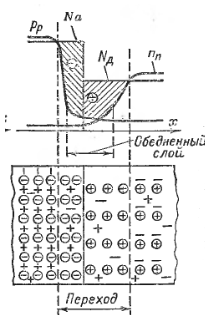
\includegraphics[scale=0.9]{p-n.png}}
		\caption{p-n переход}	
		\label{2D}
	\end{figure}
\end{center}

Т.о, на p-n переходе возникает запирающий слой. Из распределения Ферми-Дирака известно, что:
$$
F_n(E) = \frac{1}{exp\left(-\frac{E-E_f}{kT} \right) + 1}
$$

Концентрация электронов в зоне проводимости определяется интегралом
$$
n = 2\int \limits_{\varphi_c}^{\infty} P(\varphi-\varphi_c)F_n(\varphi)d\varphi
$$
2 означает, что по принципу Паули на каждом уровне могут находиться два электрона. Т.о:
$$
n = N_ce^{-\frac{\varphi_c - \varphi_F}{\varphi_T}}
$$

Величина $N_c$ есть эффективная плотность состояний в зоне проводимости. По физическому смыслу эта величина близка к плотности энергетических уровней в зоне проводимости(на 1 $\textit{см}^3$) в полосе энергий от $\varphi_c$ до $\varphi_c + \varphi_T$.

Концентрация свободных дырок в валентной зоне определяется интегралом
$$
p = 2\int \limits_{\varphi_v}^{-\infty} P(-(\varphi-\varphi_v))F_p(\varphi)(-d\varphi)
$$ 
или
$$
p = N_ve^{-\frac{\varphi_F - \varphi_v}{\varphi_T}}
$$

Величина $N_v$ есть эффективная плотность состояний в валентной зоне.

$\varphi_c$ и $\varphi_v$ есть ни что иное как потенциалы дна зоны проводимости и потолка валентной зоны соответственно. Коэффициенты $N_c$ и $N_v$ определяются по следующим формулам:
$$
N_{c/v} = 2\left(\frac{2\pi m_{n/p}q\varphi_T}{h^2}\right)^{3/2} \approx 0.5\times10^{16}\left(\frac{m_{n/p}}{m}\right)^{3/2}
$$
Тогда
\begin{equation}
n/p = exp\left[-\frac{2(\varphi_E - \varphi_F)}{\varphi_T}\right]
\label{seven}
\end{equation},
где $\varphi_E = 1/2(\varphi_c + \varphi_v)$ - потенциал середины запрещенной зоны.

$$
np = n_ip_i=n_i^2
$$

$n_i$ = $p_i$ есть концентрации электронов и дырок в собственном п/п. Тогда по (\ref{seven}) с учётом, что $p=n_i^2/n$ и $n = n_i^2/p$ получаем потенциал Ферми в двух формах:
$$
\varphi_F = \varphi_E + \varphi_Tln\frac{n}{n_i}
$$
$$
\varphi_F = \varphi_E - \varphi_Tln\frac{p}{n_i}
$$

\textbf{Контактная разность потенциалов} вводится как $\varphi_{E_p} - \varphi_{E_n}$ (см. рис.). Можно воспользоваться формулами, написанными выше и выразить $\varphi_E$ через концентрации свободных электронов в p и n-слоях.
Выразим электростатический потенциал полупроводника с тем учетом, что концентрация примесей меняется ступенькообразно.\\
$$
\varphi_{E_p} = -\varphi_Tln\frac{n_{p_0}}{n_i} + \varphi_F
$$

$$
\varphi_{E_n} = -\varphi_Tln\frac{n_{n_0}}{n_i} + \varphi_F
$$ 

\begin{center}
	\begin{figure}[h!]
		\center{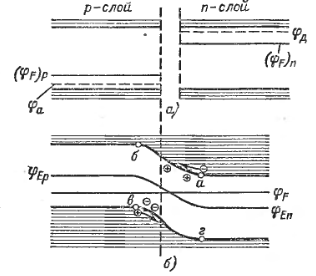
\includegraphics[scale=0.9]{zonediag.png}}
		\caption{Зонная диаграмма p-n перехода}	
		\label{2D}
	\end{figure}
\end{center}


Тогда разность электростатических потенциалов мы будем называть контактной разностью потенциалов $ \Delta \phi_0$. Из выше описанных уравнений получаем выражение контактной разности:
\begin{equation}
\Delta\varphi_0 = \varphi_Tln\frac{n_{n_0}}{n_{p_0}} = \varphi_Tln\frac{p_{p_0}}{p_{n_0}}
\end{equation}
Где $n_{n0}$ - концентрация свободных электронов в n-области в равновесном состоянии. $n_{p0}$, соответственно, в p-области.\\
Заметим, что соотношения концентраций всегда подчиняются зависимости \ref{eq:conc_ratio}, а следовательно могут быть выражены формулами \ref{eq:conc_dep}.


Можно выразить концентрацию неосновных носителей через концентрацию основных. При этом контактная разность потенциалов можно выразить через удельные сопротивления слоёв. Таким образом, при комнатной температуре для кремния можно получить величину 0.82В, а для германия 0.4В.
\pagebreak
